
%(BEGIN_QUESTION)
% Copyright 2009, Tony R. Kuphaldt, released under the Creative Commons Attribution License (v 1.0)
% This means you may do almost anything with this work of mine, so long as you give me proper credit

Read and outline the ``Analogy to Opamp Circuits'' section of the ``Pneumatic Instrumentation'' chapter in your {\it Lessons In Industrial Instrumentation} textbook.  Note the page numbers where important illustrations, photographs, equations, tables, and other relevant details are found.  Prepare to thoughtfully discuss with your instructor and classmates the concepts and examples explored in this reading.

\underbar{file i03930}
%(END_QUESTION)





%(BEGIN_ANSWER)


%(END_ANSWER)





%(BEGIN_NOTES)

Self-balancing pneumatic instruments act much like negative-feedback operational amplifier circuits, where a highly sensitive differential detector (i.e. baffle/nozzle and relay ; opamp) is used to generate an output signal, which is fed back degeneratively to its own input in order to maintain the overall gain at some precise, modest quantity.

\vskip 10pt

If the negative feedback is 100\% in strength, the resulting (overall) gain is unity (1).  This is called a ``voltage follower'' in electronics, or it could be called a ``pressure follower'' in pneumatics.  If the negative feedback is less than 100\%, the overall gain will be greater than unity.  Moreover, this overall gain will be a strong function of the feedback network (i.e. bellows and levers ; resistors) and only a weak function of the amplifier's internal gain, which means the system will behave linearly and predictably despite inevitable fluctuations in amplifier performance.

\vskip 10pt

When negative feedback is in effect, the input seen by the highly sensitive amplifier is held very nearly constant.  In fact, we may make the simplifying assumption that the amplifier's input doesn't change (i.e. baffle/nozzle gap remains essentially constant ; opamp differential input voltage remains essentially zero).  This assumption helps us analyze the system more easily, by letting us assume the amplifier output will rise or fall to {\it whatever value it must} to hold its input constant.  In other words, we assume an unchanging input, and then see what the output must do in order to attain that goal of no input change.  The result of this analysis will be very nearly what happens in real life.

\vskip 10pt

We may increase the gain of a feedback system by attenuating that negative feedback.  By feeding back a fraction of the output signal, the output signal is forced to rise to greater levels than it ordinarily would for the same input signal (i.e. a higher gain).

\vskip 10pt

Pneumatic self-balancing instruments may be broadly categorized as either {\it force-balance} or {\it motion-balance}.  In a force-balance instrument, the parts are like two sides of a perfectly balanced tug-of-war, where motion is eliminated in the act of two forces being exactly opposed.  In a motion-balance instrument, the parts are like two ballroom dancers, where motion freely occurs in complementary directions in the act of maintaining a constant gap.





\vskip 20pt \vbox{\hrule \hbox{\strut \vrule{} {\bf Suggestions for Socratic discussion} \vrule} \hrule}

\begin{itemize}
\item{} Analyze in detail the dual-bellows {\it differential-input pneumatic relay} mechanism.
\item{} Explain step-by-step the evolution of the voltage buffer equation, explaining how and why we end up with a gain of only 1 despite the opamp's incredibly high internal gain.
\item{} Identify and explain the ``simplifying assumption'' applied to the analysis of negative feedback opamp and pneumatic relay systems alike. 
\item{} Identify and explain the distinction between {\it force-balance} and {\it motion-balance} pneumatic mechanisms.
\item{} Explain how a gain other than unity (1) may be achieved for a negative-feedback system (either electronic or pneumatic).
\item{} In analyzing pneumatic self-balancing systems, we apply the simplifying assumption that the baffle/nozzle gap remains essentially constant.  Identify a real-life condition that would violate this rule; that is, would cause this gap to either increase or decrease substantially.
\end{itemize}











\vfil \eject

\noindent
{\bf Prep Quiz:}

A ``simplifying assumption'' we make about pneumatic instrument mechanisms to aid our analysis of them is:

\begin{itemize}
\item{} The nozzle cannot plug with debris because the air supply is filtered
\vskip 5pt
\item{} Motion-balance mechanisms should be used when accuracy is important
\vskip 5pt
\item{} All bellows in an instrument will exert the exact same amount of force
\vskip 5pt
\item{} Negative feedback ensures practically zero motion for all components
\vskip 5pt
\item{} There will be negligible air flow through the vent port(s)
\vskip 5pt
\item{} The baffle/nozzle gap remains constant through the action of feedback
\end{itemize}



\vfil \eject

\noindent
{\bf Summary Quiz:}

Calculate the output voltage of the following op-amp circuit, as well as the voltage at the inverting input terminal (with respect to ground):

$$\includegraphics[width=15.5cm]{i03930x01.eps}$$

\begin{itemize}
\item{} $V_{out}$ = +10 volts ; $V_{inverting}$ = +2.5 volts
\vskip 5pt
\item{} $V_{out}$ = +7.5 volts ; $V_{inverting}$ = +2.5 volts 
\vskip 5pt
\item{} $V_{out}$ = +2.5 volts ; $V_{inverting}$ = 0.833 volts 
\vskip 5pt
\item{} $V_{out}$ = +2.5 volts ; $V_{inverting}$ = 0.625 volts 
\vskip 5pt
\item{} $V_{out}$ = +10 volts ; $V_{inverting}$ = 0 volts 
\vskip 5pt
\item{} $V_{out}$ = +7.5 volts ; $V_{inverting}$ = 0 volts
\end{itemize}


%INDEX% Reading assignment: Lessons In Industrial Instrumentation, Pneumatic Instrumentation (analogy to opamp circuits)

%(END_NOTES)


